\documentclass[conference]{IEEEtran}
\IEEEoverridecommandlockouts
% The preceding line is only needed to identify funding in the first footnote. If that is unneeded, please comment it out.
\usepackage{cite}
\usepackage{listings}
\usepackage{color}
\usepackage{stfloats}
\usepackage{subfigure}
\usepackage{amsmath,amssymb,amsfonts}
\usepackage{algorithmic}
\usepackage{graphicx}
\usepackage{textcomp}
\usepackage{xcolor}
\definecolor{dkgreen}{rgb}{0,0.6,0}
\definecolor{gray}{rgb}{0.5,0.5,0.5}
\definecolor{mauve}{rgb}{0.58,0,0.82}
\lstset{frame=tb,
  language=Python,
  aboveskip=3mm,
  belowskip=3mm,
  showstringspaces=false,
  columns=flexible,
  basicstyle={\small\ttfamily},
  numbers=none,
  numberstyle=\tiny\color{gray},
  keywordstyle=\color{blue},
  commentstyle=\color{dkgreen},
  stringstyle=\color{mauve},
  breaklines=true,
  tabsize=3
}
\def\BibTeX{{\rm B\kern-.05em{\sc i\kern-.025em b}\kern-.08em
    T\kern-.1667em\lower.7ex\hbox{E}\kern-.125emX}}
\begin{document}

\title{Project B: Knowledge Distillation for Building Lightweight Deep Learning Models in Visual Classification Tasks
}
\maketitle

\begin{abstract}
This paper is a report for Project A of ECE1512 2022W, University of Toronto.
In this paper, we introduce two tasks assigned to us in detail, including the implementation and evaluation of KD based on two couples of Teacher-Student Models.
For the advanced knowledge distillation method, we choose the Early-Stopping Knowledge Distillation. We reviewed the paper 2 in the Lab Manual and implemented the corresponding methodology. Moreover, we fit the methods on different models and evaluated their performance accordingly. This project remote repository is attached on GitHub: https://github.com/Awesome-guys-in-ECE1747/ECE1512\_2022W\_ProjectRepo\_J.Xu\_and\_W.Xu
\end{abstract}

\section{Task 1: Knowledge Distillation in MNIST dataset}
In this task, we basically implement the load \& preprocess of dataset, model construction, training and evaluation for teacher and student models using our own training functions.
In addition, we implement the Early-Stopping Knowledge Distillation as the improving algorithm.
\subsection{Question 1}

In this section, we read the paper of Geoffrey Hinton\cite{b6}, and answer the assigned questions.

\subsubsection{SubQuestion a}
The purpose of using Knowledge Distillation is to compress the knowledge in an ensemble to a single model which is much easier to deploy without losing much accuracy.\par
As is widely acknowledged, in machine learning, large models usually have higher knowledge capacity than small models, thus improving state of the art on more tasks. 
However, with the increase of parameters in models, it takes more time and money to deploy, train and evaluate larger models.
In the resource-restricted systems such as mobile devices, it's hard for them to train the models. What's more, in real-time systems, although they have enough resources for training, the low efficiency means that it's inapplicable.
In order to solve it, smaller models are proposed to mimic the prediction of large models, especially in edge device such as mobile device. In a word, the goal of knowledge distillation is transferring from the teacher model to the student model and making a lightweight model that is fast, memory-efficient, and energy-efficient.

\subsubsection{SubQuestion b}
% In the paper, what knowledge is transferred from the teacher model to the student model?
The knowledge is a learned mapping from input vectors to output vectors.\par
In the previous studies, researchers tend to consider the parameters in the model as the knowledge, but it's inapplicable here. If we want to compress the model without losing too much accuracy, we have to update this concept. 
The basic nature of all the functions and models are mapping from the input to the output. 
If we want the student model which is the simple model to act like teacher while having less parameters, it means they should have similar output vectors. So both student and teacher models should have similar functions of mapping from the same input vectors to the similar output vectors.
\subsubsection{SubQuestion c}
% What is the temperature hyperparameter T? Why do we use it when transferring knowledge
% from one model to another? What effect does the temperature hyperparameter have in KD?
The temperature hyperparameter T is a parameter used to adjust the corresponding loss values for different labels in the soft targets. T makes the labels which have low probabilities influence more in the cross-entropy cost function during the transfer stage.\par
In our normal training, we only pay attention to the difference between result with highest probability and ground truth. This kind of similarity is constructed based on large amount of samples.
When the soft targets have high entropy, they'll provide much more information for the student model training than hard targets. However, in this kind of situation, the results which have a low probability contribute little to the loss functions, thus providing little information for the knowledge transferring stage.
For example, the teacher model in task1 has a high accuracy on MNIST, much of the information about the learned model is contained in the options which have very small probabilities in the soft targets. To solve it, Hinton\cite{b6} put forward the temperature hyperparameter T to magnify the corresponding loss values of low probability options.
\par
So the effect of the temperature hyperparameter is decreasing the influence of highest probability prediction and increase the influence of other labels in the knowledge transferring stage.

\subsubsection{SubQuestion d}
This is the graph of Knowledge Distillation.
\begin{figure}[h] 
    \centering
    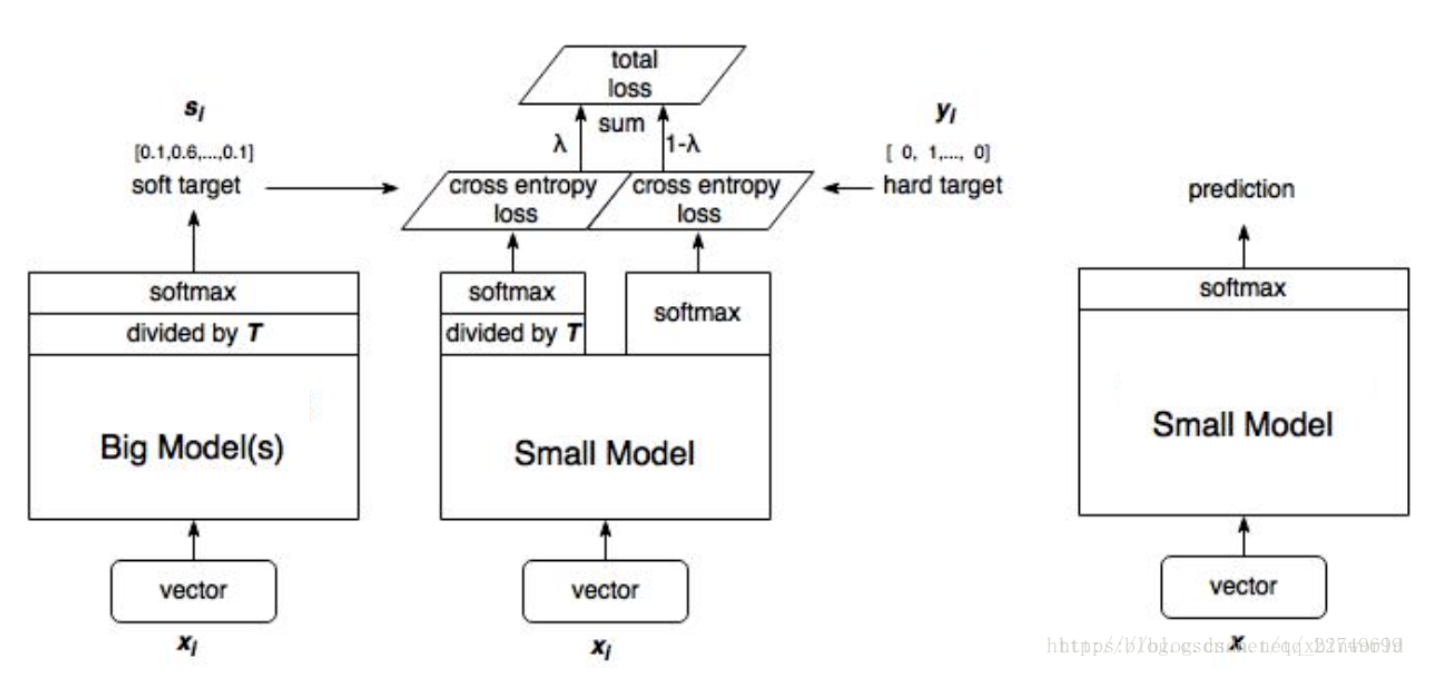
\includegraphics[width=0.45\textwidth]{./graphs/KD.png}
    \caption{Knowledge Distillation}
    \label{Fig.t1q3e}
\end{figure}
% Explain in detail the loss functions on which the teacher and student model are trained in this paper. How does the task balance parameter affect student learning? 
For the teacher model, assuming that the output vector of the final fully connection layer is $z$, then $z_{i}$ will be the logits of label $i$. 
The predicted probability for the input vector to belong to label $i$ is calculated with softmax function:
$$p_{i}=\frac{exp(z_{i})}{\sum_{j}exp(z_{j})}$$
where $p_{i}$ is the probability of being label $i$, $z_{i}$ is the logits of label $i$, $j$ is the list of all the labels.
According to it, we will calculate the loss value of teacher model like the normal neural networks. The formula is:
$$L_{teacher}=-\sum_{i}^{N}y_{i}log(p_{i})$$
where $N$ is the number of classes in total, $y_{i}$ is a Boolean value, if the sample in input vector belongs to label $i$, it'll be 1, else it'll be 0. $p_{i}$ is the predicted probability for the input vector to belong to label $i$.
\par

For the student model, we will first talk about "how does the task balance parameter affect student learning?".
The temperature hyperparameter T controls the importance and influence of every soft targets by revising the predicted probability for the input vector to belong to label $i$. The revised version of probability for label $i$ under temperature $T$, named $q_{i}^{T}$, is:
$$q_{i}^{T}=\frac{exp(z_{i}/T)}{\sum_{j}exp(z_{j}/T)}$$
where $q_{i}^{T}$ is the probability of being label $i$, $z_{i}$ is the logits of label $i$ in student model, $j$ is the list of all the labels.
Higher temperature will make the probability distribution more balanced. To be specific, suppose: $$T\to \infty $$, then every labels will have the same probabilities. 
On the contrary, if $$T\to 0 $$ soft targets will become one-hot tensor, which is named "hard targets".\par
Let's continue to talk about the loss value of student model. The traditional knowledge distillation is the combination of both the student loss and distillation loss.
The formula for the combination is:
$$L=\alpha L_{soft}+\beta L_{hard}$$
where $L_{soft}$ is the distill loss (corresponding to soft targets) and student loss (corresponding to hard targets). $\alpha$ is the weight of $L_{soft}$ which is defined manually, and $\beta$ is the weight of $L_{hard}$ which equals $(1-\alpha)$ here.
For the student loss, it should be similar to teacher model. This is named $L_{hard}$ for it's the hard targets loss of the student model. The formula is:
$$L_{hard}=-\sum_{i}^{N}y_{i}log(q_{i}^{1})$$
where $N$ is the number of classes in total, $y_{i}$ is a Boolean value, if the sample in input vector belongs to label $i$, it'll be 1, else it'll be 0. $q_{i}^{1}$ is the predicted probability for the input vector to belong to label $i$ in temperature $1$.
For the soft targets loss, the formula is:
$$L_{soft}=-\sum_{i}^{N}p_{i}^{T}log(q_{i}^{T})$$
where $N$ is the number of classes in total, $p_{i}^{T}$ is the predicted probability for the input vector in teacher model to belong to label $i$ in temperature $T$, $q_{i}^{T}$ is the predicted probability for the input vector in student model to belong to label $i$ in temperature $T$.
To explain $p_{i}^{T}$ in detail, we listed the formula too:
$$p_{i}^{T}=\frac{exp(v_{i}/T)}{\sum_{j}exp(v_{j}/T)}$$
where $p_{i}^{T}$ is the probability of being label $i$, $v_{i}$ is the logits of label $i$ in teacher model, $j$ is the list of all the labels.
\subsubsection{SubQuestion e}
% Can we look at the KD as a regularization technique, here? Explain your rationale.
From our perspective, the knowledge distillation can be considered as a regularization technique. As is illustrated in the paper\cite{b6}, we can use soft targets to prevent overfitting. It's the same effect as regularization.
In an unbalanced dataset, assume one of the classes named 'A' has many more samples than other classes, it's highly likely that the model with a full softmax layer over all classes will be overfitting on this special class A.
The reason is that: if there are more samples of class A in the input, more information will be applied into the model, thus making the information of other classes which have low predicted possibilities become less important. 
However, the information in these low possibilities in the soft labels is very important. They contains the information which traditional one-hot labels don't have. 
\par
In contrast, if we use soft targets of knowledge distillation as the training targets, we can prevent class A from passing too much information into the model, thus making the information of other labels which have low possibilities more important.
If we adjust the hyperparameters carefully, we can get balanced information from both the large-sized labels and small-sized labels, which will lead to the good performance of the model. It's the same as regularization technique.

\subsection{Question 2}
In this section, we build a cumbersome teacher and a lightweight student model training on MNIST dataset. The network structure is plotted by $model:summary()$.
The teacher model contains two convolutional layers with relu function, two max-pooling layers, a flatten layer and two dense layers. It's not a complex network, the implementation code is as followed.
\begin{lstlisting}
    from keras.models import Sequential
    from keras.layers import Input, Conv2D, MaxPooling2D, Dense, Flatten, Dropout
    
    # print(mnist_test)
    
    # Build CNN teacher.
    def build_cnn():
      cnn_model = Sequential()
      cnn_model.add(Input((28,28,1)))
      cnn_model.add(Conv2D(filters=32, kernel_size=(3,3), strides= (1,1), activation='relu'))
      cnn_model.add(MaxPooling2D(pool_size=(2,2), strides= (1,1)))
      cnn_model.add(Conv2D(filters=64, kernel_size=(3,3), strides= (1,1), activation='relu'))
      cnn_model.add(MaxPooling2D(pool_size=(2,2), strides= (2,2)))
      cnn_model.add(Flatten())
      cnn_model.add(Dropout(rate=0.5))
      cnn_model.add(Dense(units=128, activation='relu'))
      cnn_model.add(Dropout(rate=0.5))
      cnn_model.add(Dense(NUM_CLASSES, activation='softmax'))
      return cnn_model
    
    cnn_model=build_cnn()
    print("\n\n\n============ Teacher Model ============\n")
    cnn_model.summary()
\end{lstlisting} \par
The screenshot of teacher model is shown below:
\begin{figure}[h] 
    \centering
    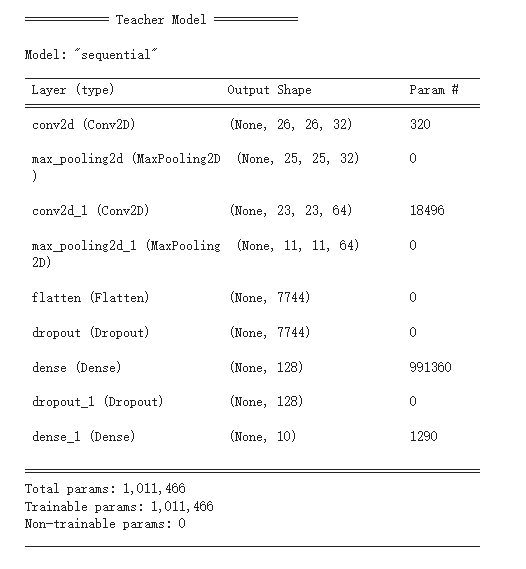
\includegraphics[width=0.45\textwidth]{./graphs/Teacher_MNIST.png}
    \caption{Teacher Model}
    \label{Fig.t1q3e}
\end{figure}
The student model contains a flatten layer and three dense layers.The code is listed as below:
\begin{lstlisting}
# Build fully connected student.
def build_fc():
  fc_model = Sequential()
  fc_model.add(Input((28,28,1)))
  fc_model.add(Flatten())
  fc_model.add(Dense(units=784,activation='relu'))
  fc_model.add(Dense(units=784,activation='relu'))
  fc_model.add(Dense(NUM_CLASSES, activation='softmax'))
  return fc_model
fc_model=build_fc()
print("\n\n\n============ Student Model ============\n")
fc_model.summary()
\end{lstlisting} \par
The screenshot of student model summary is shown below:
\begin{figure}[h] 
    \centering
    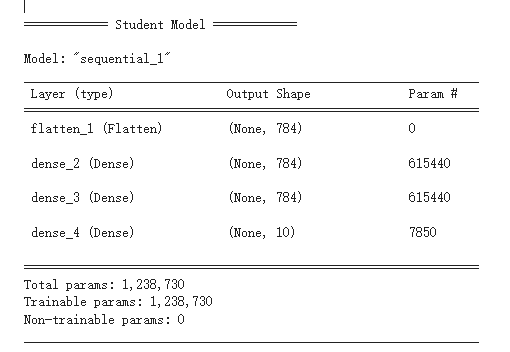
\includegraphics[width=0.45\textwidth]{./graphs/Student_MNIST.png}
    \caption{Student Model}
    \label{Fig.t1q3e}
\end{figure}
\subsection{Question 3}
In this section, we will talk about the implementation of loss functions in teacher and student models, consisting of three parts.\par
The first part is the loss function for teacher model. The code is shown below.\par 
We first calculated the logits of teacher model using the input images. Then we call the function in tensorflow $tf.nn.sparse_softmax_cross_entropy_with_logits$ to calculate the cross-entropy loss with logits. 
The logits parameter is the $subclass_logits$ which is calculated above, and the label is $tf.argmax(labels, 1)$, since the $labels$ is a 1D vector which has 10 elements. In the vector, only the true label is set to 1 while others are set to 0.
As a result, $tf.argmax(labels, 1)$ is the true label.
\begin{lstlisting}
@tf.function
def compute_teacher_loss(images, labels):
  """Compute subclass knowledge distillation teacher loss for given images
     and labels.

  Args:
    images: Tensor representing a batch of images.
    labels: Tensor representing a batch of labels.

  Returns:
    Scalar loss Tensor.
  """
  subclass_logits = cnn_model(images, training=True)
  # print(subclass_logits.shape)
  # print(tf.argmax(labels, 1).shape)
  # Compute cross-entropy loss for subclasses.

  # your code start from here for step 3
  cross_entropy_loss_value = tf.nn.sparse_softmax_cross_entropy_with_logits(logits=subclass_logits, labels=tf.argmax(labels, 1))


  return cross_entropy_loss_value
\end{lstlisting}
The second part is the $distillation_loss$ function. 
In this function, we first define the $\alpha$ and the temperature $T$ according to the requirement in the lab manual.
Then we calculated the soft targets according to the formula above and the softmax function.
After that, we will calculate the cross-entropy loss like the teacher model loss.
At last, we calculated the average number of cross-entropy multiply $T_{2}$ as the soft targets loss value, named $L_{soft}$.\par
The code is shown below.
\begin{lstlisting}
# Hyperparameters for distillation (need to be tuned).
ALPHA = 0.5 # task balance between cross-entropy and distillation loss
DISTILLATION_TEMPERATURE = 4. # temperature hyperparameter
import numpy as np
import torch
import torch.nn as nn
def distillation_loss(teacher_logits: tf.Tensor, student_logits: tf.Tensor,
                      temperature: Union[float, tf.Tensor]):
  """Compute distillation loss.

  This function computes cross entropy between softened logits and softened
  targets. The resulting loss is scaled by the squared temperature so that
  the gradient magnitude remains approximately constant as the temperature is
  changed. For reference, see Hinton et al., 2014, "Distilling the knowledge in
  a neural network."

  Args:
    teacher_logits: A Tensor of logits provided by the teacher.
    student_logits: A Tensor of logits provided by the student, of the same
      shape as `teacher_logits`.
    temperature: Temperature to use for distillation.

  Returns:
    A scalar Tensor containing the distillation loss.
  """
  # print(tf.reduce_sum(tf.exp(teacher_logits/temperature),axis=1,keepdims=True).shape)
  soft_targets = tf.exp((teacher_logits-np.max(teacher_logits,axis=-1,keepdims=True))/temperature)/tf.reduce_sum(tf.exp(np.max(teacher_logits,axis=-1,keepdims=True)/temperature),axis=1,keepdims=True)

  return tf.reduce_mean(tf.nn.softmax_cross_entropy_with_logits(soft_targets, student_logits / temperature)) * temperature ** 2

\end{lstlisting}
The thrid part is the student loss which combines both $L_{hard}$ and $L_{soft}$.First, we calculate the logits for student model as $student_subclass_logits$ and logits for taecher model as $teacher_subclass_logits$.
Then we call the $distillation_loss$ function defined above to calculate the soft targets loss value $L_{soft}$.
After that, we calculate the $L_{hard}$ like the teacher loss. We use the $tf.nn.sparse_softmax_cross_entropy_with_logits$ function to compute the student hard loss.
At last, for the overall loss value, we calculate the combination of $L_{hard}$ and $L_{soft}$ with their weights accordingly.\par
The code is shown below:
\begin{lstlisting}
def compute_student_loss(images, labels):
  """Compute subclass knowledge distillation student loss for given images
     and labels.

  Args:
    images: Tensor representing a batch of images.
    labels: Tensor representing a batch of labels.

  Returns:
    Scalar loss Tensor.
  """
  student_subclass_logits = fc_model(images, training=True)

  # Compute subclass distillation loss between student subclass logits and
  # softened teacher subclass targets probabilities.

  teacher_subclass_logits = cnn_model(images, training=False)
  distillation_loss_value = distillation_loss(teacher_subclass_logits,student_subclass_logits,DISTILLATION_TEMPERATURE)
  L_hard=tf.nn.sparse_softmax_cross_entropy_with_logits(logits=student_subclass_logits, labels=tf.argmax(labels, 1))
  # print(labels)
  # Compute cross-entropy loss with hard targets.

  cross_entropy_loss_value = ALPHA*distillation_loss_value+(1-ALPHA)*L_hard

  return cross_entropy_loss_value
\end{lstlisting}

\subsection{Question 4}
In this section, we complete the $train_and_evaluate$ function.
First, we define the optimizer with $Adam$ and set learning rate as $0.001$.
Then we use a for loop to simulate the training process in tensorflow library.
In the each epoch, we calculate the loss value by calling the $compute_loss_fn$ function and pass in the images and corresponding labels in the training batch.
The $compute_loss_fn$ function is the loss function name passed in.
Then we will apply the loss values to compute the gradients with function $tape.gradient$. 
After that, we will apply the gradients to modify the model's variables.
At the end of the epoch, we call the $compute_num_correct$ function to evaluate the performance of this training epoch.\par
The code is listed below.
\begin{lstlisting}
    def train_and_evaluate(model, compute_loss_fn):
    """Perform training and evaluation for a given model.
  
    Args:
      model: Instance of tf.keras.Model.
      compute_loss_fn: A function that computes the training loss given the
        images, and labels.
    """
    optimizer = tf.keras.optimizers.Adam(learning_rate=0.001)
    res=0.0
    for epoch in range(1, NUM_EPOCHS + 1):
      # Run training.
      print('Epoch {}: '.format(epoch), end='')
      for images, labels in mnist_train:
        with tf.GradientTape() as tape:
          loss_value = compute_loss_fn(images,labels)
  
        grads = tape.gradient(loss_value,model.variables)
        optimizer.apply_gradients(zip(grads, model.variables))
  
      # Run evaluation.
      num_correct = 0
      num_total = builder.info.splits['test'].num_examples
      for images, labels in mnist_test:
        num_correct += tf.cast(compute_num_correct(model,images,labels)[0],tf.int32)
      print("Class_accuracy: " + '{:.2f}%'.format(
          num_correct / num_total * 100))
      res=num_correct / num_total * 100
    return res
      
\end{lstlisting}
\subsection{Question 5}
For the first part, we will talk about the training and test accuracy of the teacher amd student model.
First is the teacher model, we just call the $train_and_evaluate$ function. The code is listed below.
\begin{lstlisting}
# your code start from here for step 5 
train_and_evaluate(cnn_model,compute_teacher_loss)
\end{lstlisting}
The screenshot of the accuracy is shown below.

\begin{figure}[h] 
    \centering
    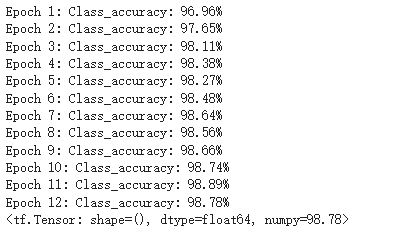
\includegraphics[width=0.45\textwidth]{./graphs/teacher_accuracy_mnist.png}
    \caption{Teacher Model Testing Accuracy}
    \label{Fig.t1q3e}
\end{figure}
Second is the student model, since we need to tune the distillation hyperparameters, we used a loop to do it.
We set the parameter temperature to $1,2,4,16,32,64$ and set alpha to $0.1,0.3,0.5,0.7,0.9$. In total, we trained 30 models.
The code is shown below.
\begin{lstlisting}
T=[1,2,4,16,32,64]
A=[0.1,0.3,0.5,0.7,0.9]
y=[]
for i in T:
  for j in A:
    DISTILLATION_TEMPERATURE = i # Temperature hyperparameter
    ALPHA=j
    fc_model=build_fc()
    print('temperature:'+str(i)+' Alpha:'+str(j))
    acu=train_and_evaluate(fc_model,compute_student_loss)
    fc_model.save('student_MNIST_t'+str(i)+'a'+str(j)+'.h5')
    y.append(acu)
# train_and_evaluate(fc_model,compute_student_loss)
\end{lstlisting}
Then we print out the training accuracy stored with the code below.
\begin{lstlisting}
# fc_model.save('student_MNIST_4.h5')
for i in range(6):
  for j in range(5):
    print('Temperature:'+str(i)+' Alpha:'+str(j)+' Accuracy:'+str(y[i*5+j]))
\end{lstlisting}

Here is the screenshot of testing results.
\begin{figure}[h] 
    \centering
    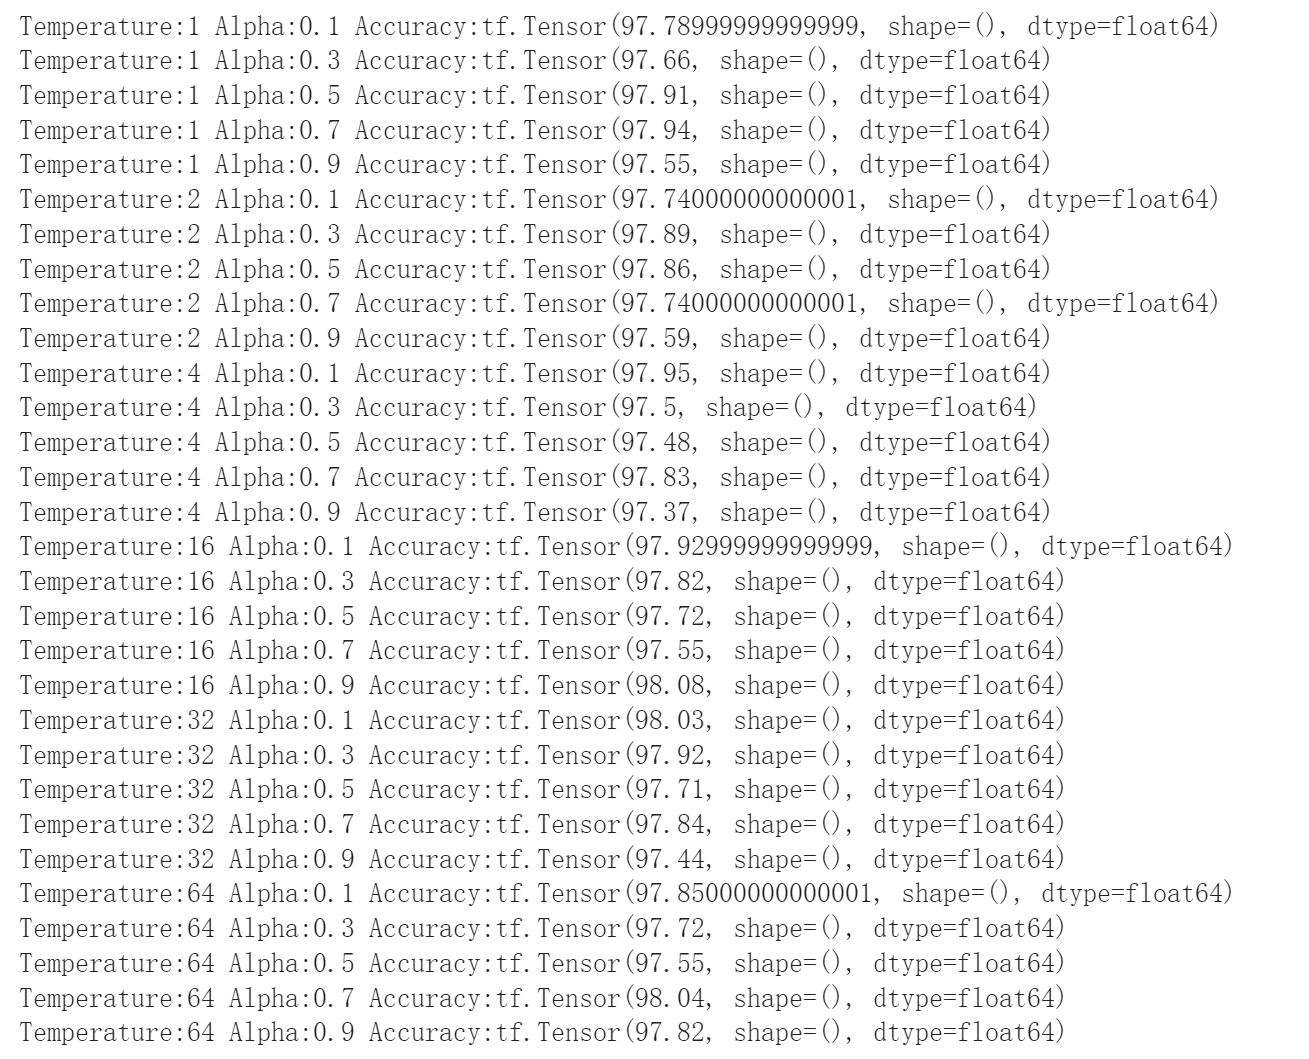
\includegraphics[width=0.45\textwidth]{./graphs/student_accuracy_mnist.png}
    \caption{Teacher Model Testing Accuracy}
    \label{Fig.t1q3e}
\end{figure}
And here is the test accuracy table for the hyperparameter tuning procedure.
\begin{table}[]
    \begin{tabular}{|l|l|l|}
    \hline
    Temperature & Alpha & Test Accuracy      \\ \hline
    1           & 0.1   & 97.78999999999999  \\ \hline
    1           & 0.3   & 97.66 \\ \hline
    1           & 0.5   & 97.91   \\ \hline
    1           & 0.7   & 97.94 \\ \hline
    1           & 0.9   & 97.55  \\ \hline
    2           & 0.1   & 97.74000000000001 \\ \hline
    2           & 0.3   & 97.89 \\ \hline
    2           & 0.5   & 97.86 \\ \hline
    2           & 0.7   & 97.74000000000001  \\ \hline
    2           & 0.9   & 97.59  \\ \hline
    4           & 0.1   & 97.95 \\ \hline
    4           & 0.3   & 97.5 \\ \hline
    4           & 0.5   & 97.48 \\ \hline
    4           & 0.7   & 97.83  \\ \hline
    4           & 0.9   & 97.37 \\ \hline
    16          & 0.1   & 97.92999999999999 \\ \hline
    16          & 0.3   & 97.82 \\ \hline
    16          & 0.5   & 97.72  \\ \hline
    16          & 0.7   & 97.55 \\ \hline
    16          & 0.9   & 98.08  \\ \hline
    32          & 0.1   & 98.03 \\ \hline
    32          & 0.3   & 97.92  \\ \hline
    32          & 0.5   & 97.71 \\ \hline
    32          & 0.7   & 97.84 \\ \hline
    32          & 0.9   & 97.44   \\ \hline
    64          & 0.1   & 97.85000000000001 \\ \hline
    64          & 0.3   & 97.72 \\ \hline
    64          & 0.5   & 97.55 \\ \hline
    64          & 0.7   & 98.04 \\ \hline
    64          & 0.9   & 97.82  \\ \hline
    \end{tabular}
    \end{table}
As is shown in the table, we think that the best alpha should be 16, and the best temperature is 0.9. However, as we can see here in the table, the hyperparameters do not affect the test accuracy too much. The variance is smaller than 1\%. So we can conclude that the adjustment of hyperparameter does not help a lot for the student models to improve their accuracy and mimic the predictions of the teacher model. It's highly possible that the difference is jitters of in the training.
\subsection{Question 6}
In this section, we will talk about the plot of a curve which is student test accuracy versus temperature hyperparameters. 
According to the requirement in the Lab Manual, we set the task balance parameter $\alpha$ as 0.5, and use a loop to change the temperature in the list.
In every loop, we change the temperature, reset the model and retrain it. The code is shown below.
\begin{lstlisting}
T=[1,2,4,16,32,64]
y=[]
for i in T:
  DISTILLATION_TEMPERATURE = i # Temperature hyperparameter
  fc_model=build_fc()
  print('temperature:'+str(i))
  acu=train_and_evaluate(fc_model,compute_student_loss)
  fc_model.save('student_MNIST_'+str(i)+'.h5')
  y.append(acu)
\end{lstlisting}
The screenshot of the training and testing is shown here.
\begin{figure}[h] 
    \centering
    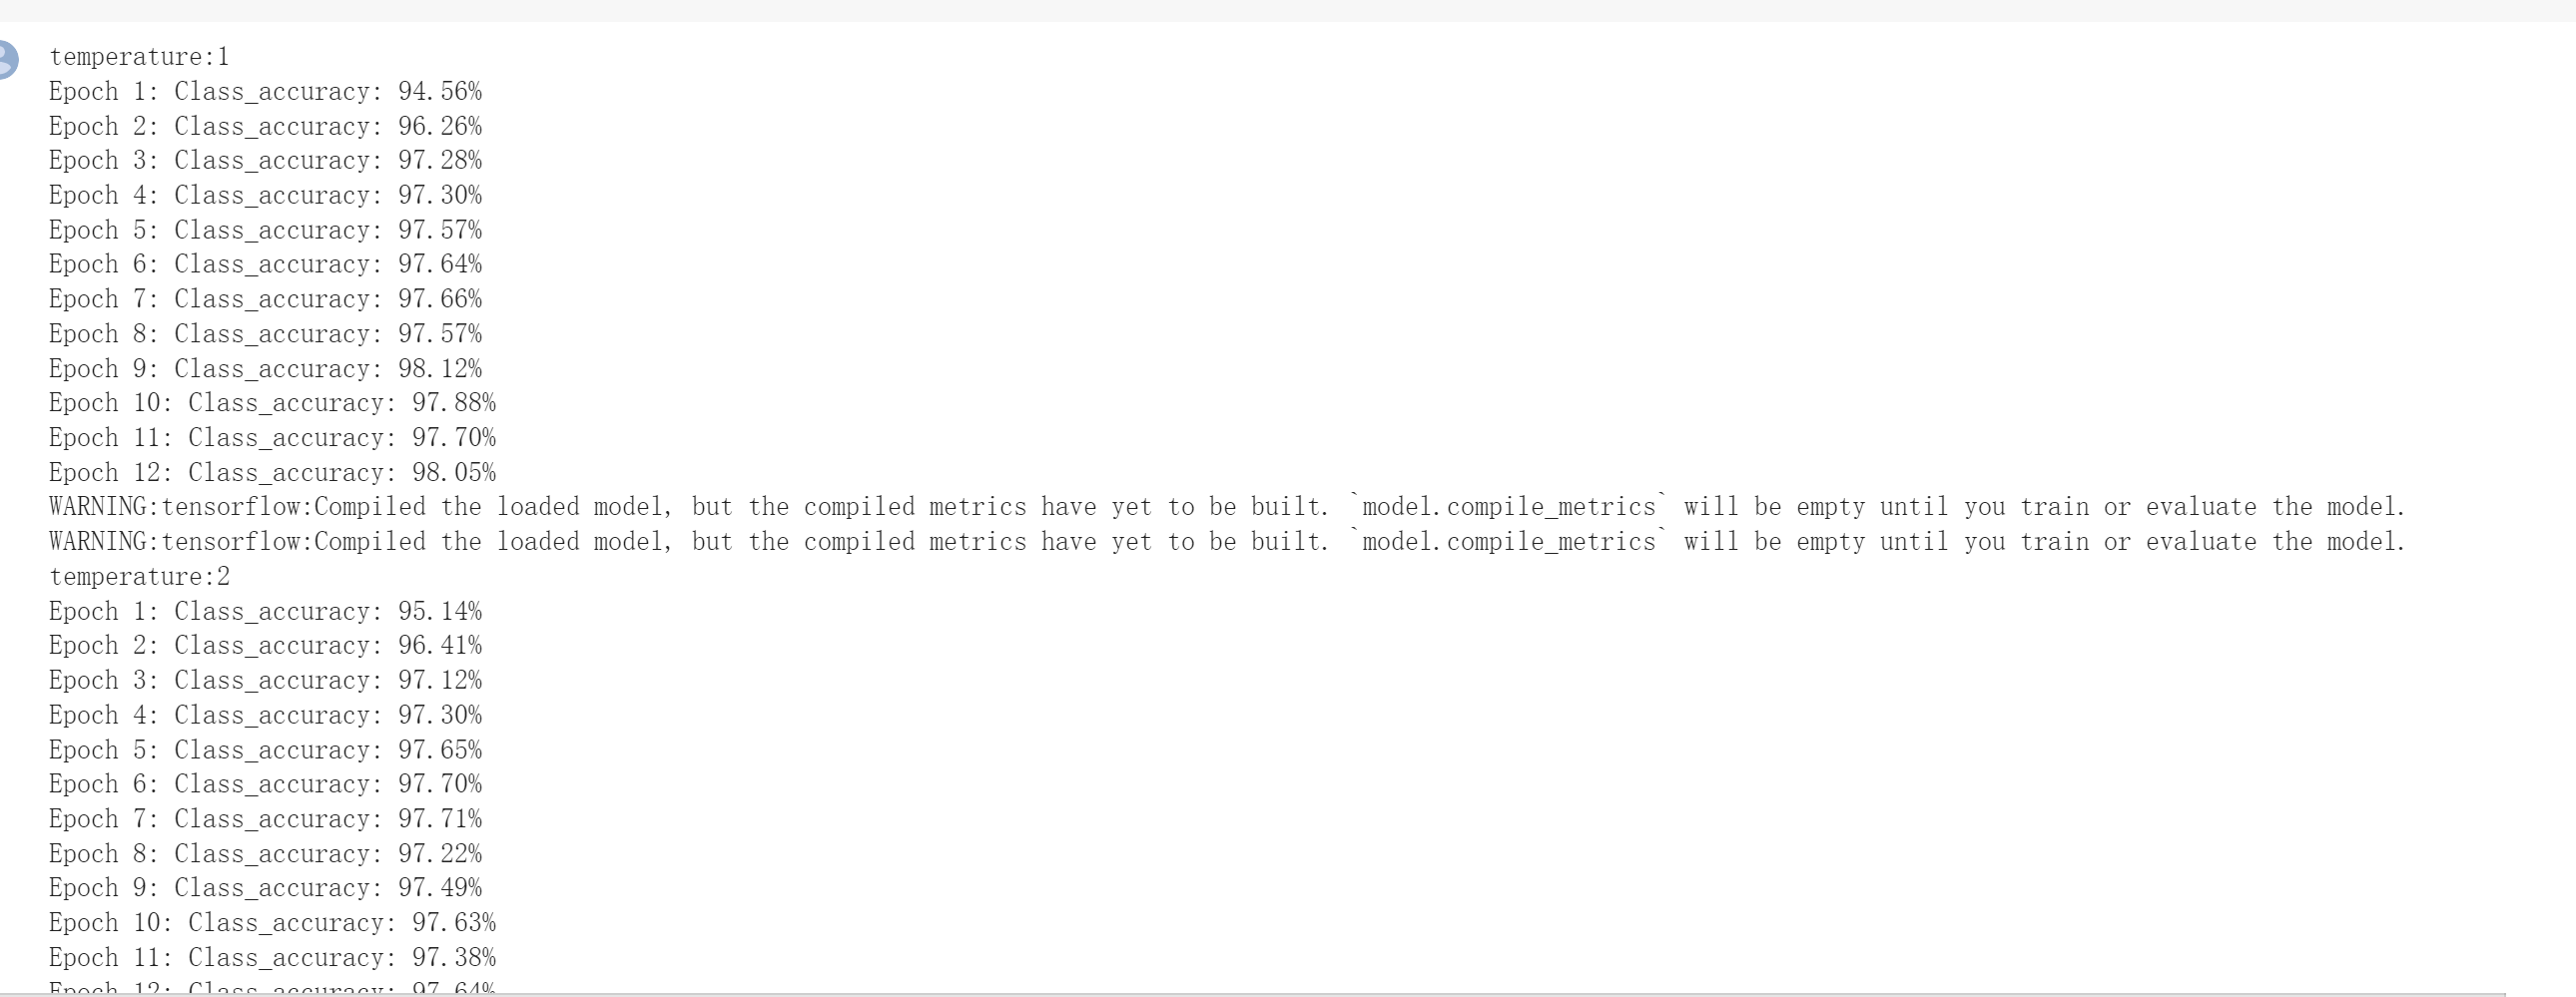
\includegraphics[width=0.45\textwidth]{./graphs/T1Q6_train.png}
    \caption{Training and testing procedure}
    \label{Fig.t1q3e}
\end{figure}
Then we use $matplotlib.pyplot$ library to plot the curve.
The code is like below.
\begin{lstlisting}
import matplotlib.pyplot as plt
x=['1','2','4','16','32','64']
l=plt.plot(x,y)
plt.title('Test accuracy vs. tempreture curve')
plt.xlabel('temperature')
plt.ylabel('test_accuracy')
plt.legend()
plt.show()
\end{lstlisting}
The curve is shown here.
\begin{figure}[h] 
    \centering
    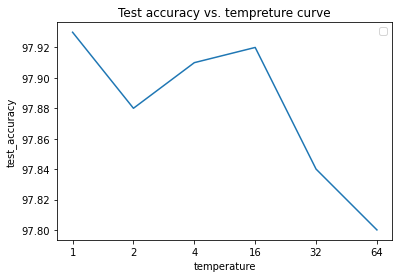
\includegraphics[width=0.45\textwidth]{./graphs/accuracy_vs_temperature.png}
    \caption{Student Accuracy VS. Temperature}
    \label{Fig.t1q3e}
\end{figure}
As is clearly shown in the picture, the accuracy decreases in general, but it does not decrease a lot.
The reason for decreasing is that: As we have stated above, with a high temperature,
% TODO: explain here
\subsection{Question 7}
In this section, we will train the student model from scratch without using Knowledge Distillation.
We will firstly create a new model. In the loss function for the student, we will calculate the logits, and pass it into the $tf.nn.sparse_softmax_cross_entropy_with_logits$ function like we do in teacher model.
Then we will pass this function into $train_and_evaluate$ function to do the training.\par
The code is shown here.
\begin{lstlisting}
# Build fully connected student.
# fc_model_no_distillation = tf.keras.Sequential()
fc_model_no_distillation = build_fc()

def compute_plain_cross_entropy_loss(images, labels):
  """Compute plain loss for given images and labels.

  For fair comparison and convenience, this function also performs a
  LogSumExp over subclasses, but does not perform subclass distillation.

  Args:
    images: Tensor representing a batch of images.
    labels: Tensor representing a batch of labels.

  Returns:
    Scalar loss Tensor.
  """
  # your code start from here for step 7
  student_subclass_logits = fc_model_no_distillation(images, training=True)
  cross_entropy_loss = tf.nn.sparse_softmax_cross_entropy_with_logits(logits=student_subclass_logits, labels=tf.argmax(labels, 1))

  
  return cross_entropy_loss


train_and_evaluate(fc_model_no_distillation, compute_plain_cross_entropy_loss)
\end{lstlisting}
The screenshot of the test accuracy is shown below.

\begin{figure}[h] 
    \centering
    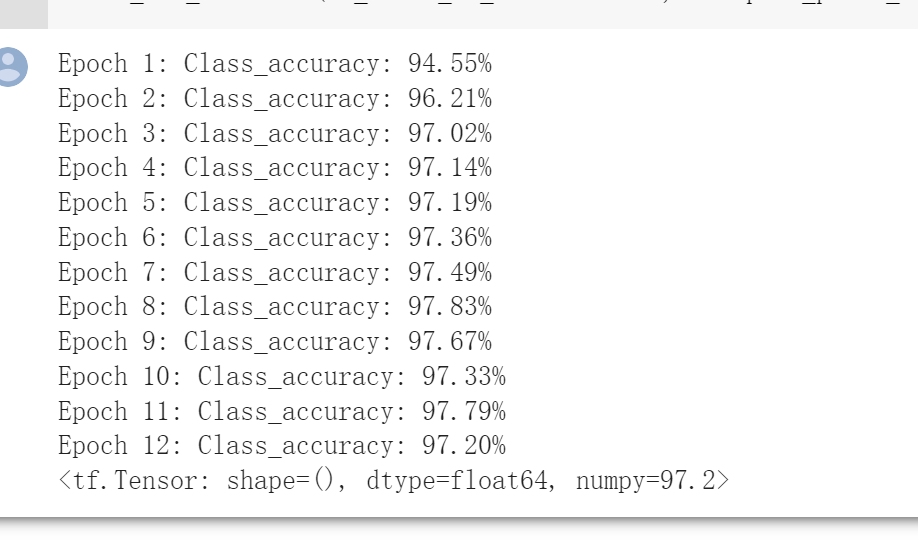
\includegraphics[width=0.45\textwidth]{./graphs/T1Q7_train.png}
    \caption{Test Accuracy of the Student Model without KD}
    \label{Fig.t1q3e}
\end{figure}
As we can see here, the test accuracy of students model with knowledge distillation is, while student model without knowledge distillation achieves $97.20\%$ accuracy in the final epoch.
So the test accuracy of student models with knowledge distillation is higher than that of student model without knowledge distillation. (For fair comparison, we set the epoch to 12.)

\subsection{Question 8}
In this part, we compute the number of parameters and FLOPs(floating-point operations per second) in teacher model and student model
We use an open-source library called $keras_flops$ to do that. We first install this library with a command line.
\begin{lstlisting}
    !pip install keras_flops
\end{lstlisting}
Then we call the functions in the library to do the calculation. For the number of parameters, we use compute it by adding up the number in every variables.
For the FLOPs, we call the library function which is $get_flops$ like the examples given in the document.
The code is shown below.
\begin{lstlisting}
    from keras_flops import get_flops
    # flops = tf.profiler.profile(fc_model, options=tf.profiler.ProfileOptionBuilder.float_operation())
    print('teacher model:')
    print('Parameter number:'+str(np.sum([np.prod(vp.get_shape().as_list()) for vp in cnn_model.variables])))
    print('FlOPs:'+str(get_flops(cnn_model,batch_size=BATCH_SIZE)/1000000000.0))
    print('student model:')
    print('Parameter number:'+str(np.sum([np.prod(vp.get_shape().as_list()) for vp in fc_model.variables])))
    print('FlOPs:'+str(get_flops(fc_model,batch_size=BATCH_SIZE)/1000000000.0))
    print('student model:')
    print('Parameter number:'+str(np.sum([np.prod(vp.get_shape().as_list()) for vp in fc_model_no_distillation.variables])))
    print('FlOPs:'+str(get_flops(fc_model_no_distillation,batch_size=BATCH_SIZE)/1000000000.0))
    # flops = tf.profiler.experimental.Profile(cnn_model, options=tf.profiler.ProfileOptionBuilder.float_operation())
    # params = tf.profiler.profile(cnn_model, options=tf.profiler.ProfileOptionBuilder.trainable_variables_parameter())
    # print('student model:')
    # flops = tf.profiler.profile(fc_model, options=tf.profiler.ProfileOptionBuilder.float_operation())
    # params = tf.profiler.profile(fc_model, options=tf.profiler.ProfileOptionBuilder.trainable_variables_parameter())
\end{lstlisting}
The result screenshot is shown here.

\begin{figure}[h] 
    \centering
    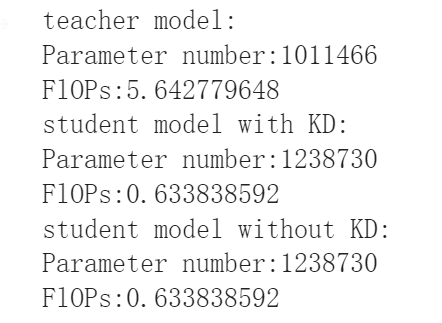
\includegraphics[width=0.45\textwidth]{./graphs/T1Q8.png}
    \caption{Parameter Number and FLOPs}
    \label{Fig.t1q3e}
\end{figure}
From the screenshot, we can see that the teacher model has parameters and FLOPs is times/second. 
The student model with KD has parameters, and FLOPs is times/second. 
The student model without KD has parameters, and FLOPs is times/second. 
\subsection{Question 9}
In this part, we will talk about our XAI methodology used to build the explanation map for the models.
\subsection{Question 10}
In this part, we read Jang Hyun Cho and Bharath Hariharan's\cite{b2} paper. The novel idea is.
\subsection{Question 11}
How does the proposed method improve the student performance in comparison to the conventional KD?
\subsection{Question 12}
What are some limitations of the proposed method? How can they be addressed?
\subsection{Question 13}
In this part, we implement the Early-Stopping Knowledge Distillation.
\begin{lstlisting}
def train_and_evaluate_ESKD(model, compute_loss_fn,epoch_num=12):
  """Perform training and evaluation for a given model.

  Args:
    model: Instance of tf.keras.Model.
    compute_loss_fn: A function that computes the training loss given the
      images, and labels.
  """

  # your code start from here for step 4
  optimizer = tf.keras.optimizers.Adam(learning_rate=0.001)
  res=0.0
  for epoch in range(1, epoch_num + 1):
    # Run training.
    print('Epoch {}: '.format(epoch), end='')
    loss_total=0
    count_total=0
    for images, labels in mnist_train:
      with tf.GradientTape() as tape:
        loss_value = compute_loss_fn(images,labels)
      grads = tape.gradient(loss_value,model.variables)
      optimizer.apply_gradients(zip(grads, model.variables))
    # Run evaluation.
    num_correct = 0
    num_total = builder.info.splits['test'].num_examples
    for images, labels in mnist_test:
      num_correct += tf.cast(compute_num_correct(model,images,labels)[0],tf.int32)
    print("Class_accuracy: " + '{:.2f}%'.format(
        num_correct / num_total * 100))
    res=num_correct / num_total * 100
  return res
\end{lstlisting}
\begin{lstlisting}
T=[1,2,3,4,5,6,7,8,9,10,11,12]
y=[]
for i in T:
  # NUM_EPOCHS = 3 #temperature hyperparameter
  cnn_model=build_cnn()
  fc_model=build_fc()
  print('EpochNumber: '+str(i))
  print('Training teacher')
  @tf.function
  def compute_teacher_loss(images, labels):
    """Compute subclass knowledge distillation teacher loss for given images
      and labels.

    Args:
      images: Tensor representing a batch of images.
      labels: Tensor representing a batch of labels.

    Returns:
      Scalar loss Tensor.
    """
    subclass_logits = cnn_model(images, training=True)
    # print(subclass_logits.shape)
    # print(tf.argmax(labels, 1).shape)
    # Compute cross-entropy loss for subclasses.

    # your code start from here for step 3
    cross_entropy_loss_value = tf.nn.sparse_softmax_cross_entropy_with_logits(logits=subclass_logits, labels=tf.argmax(labels, 1))
    return cross_entropy_loss_value
  train_and_evaluate_ESKD(cnn_model,compute_teacher_loss,i)
  # NUM_EPOCHS = 12
  print('Training student')
  acu=train_and_evaluate(fc_model,compute_student_loss)
  cnn_model.save('teacher_MNIST_ESKD_'+str(i)+'.h5')
  fc_model.save('student_MNIST_ESKD_'+str(i)+'.h5')
  y.append(acu)
\end{lstlisting}
\begin{lstlisting}
import matplotlib.pyplot as plt
x=T
l=plt.plot(x,y)
plt.title('Test accuracy vs. Teacher Epoch Number')
plt.xlabel('Teacher_epoch_number')
plt.ylabel('test_accuracy')
plt.legend()
plt.show()
\end{lstlisting}
\section{Task 2: Knowledge Distillation in MHIST dataset}

\subsection{Question 1}
\subsubsection{SubQuestion a} \textbf{How can we adapt these models for the MHIST dataset using transfer learning? Talk about the Feature Extraction and Fine-Tuning processes during transfer learning.}\\

The core idea of Transfer learning is consists of taking features learned on one problem, and leveraging them on a new, similar problem.\cite{keras}
Feature Extraction is 
\\
Fine tuning
%%%%%%%%%%
\cite{blog}
\subsubsection{SubQuestion b} \textbf{What is a residual block in ResNet architectures?}
The residual block is the significant and elemental component of ResNet, Residual Network, an example is shown in figure \label{res}.

\begin{figure}[h] 
    \centering
    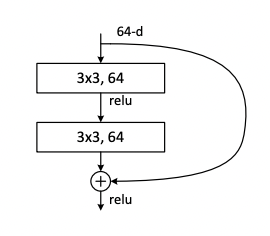
\includegraphics[width=0.3\textwidth]{./graphs/Task2/res-block.png}
    \caption{Residual Block Example}
    \label{res}
\end{figure}

A common sense of Convolutional Neural Network is that, when the depth of CNN becomes essentially deep, in which the network could be called DNN, Deep Neural Network. It will be hard to train the network model due to the problem of gradient disappearance (vanishing gradient problem) and gradient explosion. He et al.\cite{resnet} proposed ResNet whose layer could get activated with skip connection, which is like a shortcut to the deeper layers. This structure is called residual block. For example, we assume that there's an input, $a^{[l]}$, two convolution layers, with a hidden value between, $a^{[l+1]}$, and an output, $a^{[l+2]}$, shown in the figure \ref{resex}\cite{wu}.

\begin{figure}[h] 
    \centering
    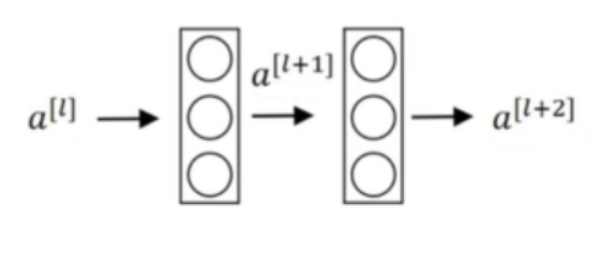
\includegraphics[width=0.45\textwidth]{./graphs/Task2/resnet-example.png}
    \caption{2-Layer Structure}
    \label{resex}
\end{figure}

In the classic CNN, we need to pass convolutional layer twice in order to compute $a^{[l+2]}$ by $a^{[l]}$, like the following formulas, where $g()$ stands for activation function, e.g. ReLU.

$$z^{[l+1]}=W^{[l+1]}a^{[l]}+b^{[l+1]}, a^{[l+1]}=g(z^{[l+1]})$$
$$z^{[l+2]}=W^{[l+2]}a^{[l+1]}+b^{[l+2]}, a^{[l+2]}=g(z^{[l+2]})$$
However, once we enable the skip connection, we are able to compute $a^{[l+2]}$ by $a^{[l]}$ with the following formula.

$$a^{[l+2]}=g(z^{[l+2]}+a^{[l]})$$
And the whole structure is a basic example of residual block. It will significantly solve the trouble of deep learning, and networks with the structure, residual block, could be able to contain more layers.

\subsubsection{SubQuestion c} \textbf{What are the differences between the ResNetV1 and ResNetV2 architectures?}

ResNetV2 is an improved version of ResNetV1, and there are three major differences between ResNetV1 and ResNetV2. Firstly, the structure of residual block is different, shown in figure \ref{resv1v2}.\cite{v1v2} ResNetV1 use the structure of \textit{Conv-BN-ReLU} and ResNetV2 use the structure of \textit{BN-ReLu-Conv}.

\begin{figure}[h] 
    \centering
    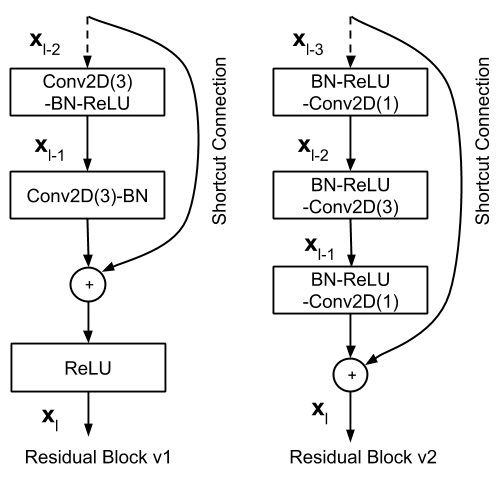
\includegraphics[width=0.45\textwidth]{./graphs/Task2/v1v2.png}
    \caption{Residual Block Structure of ResNetV1 vs. ResNetV2}
    \label{resv1v2}
\end{figure}

Secondly, the stride strategy is different. ResNetV1 keep the size of feature map of \textit{Block1(Conv2\_*)}, and ResNetV2 keep the size of feature map of \textit{Block4(Conv5\_*)}. Thirdly, ResNetV2 enhance the regularization by using pre-activation, so the model will be trained faster.

\subsubsection{SubQuestion d} \textbf{What are the differences between the MobileNetV1 and MobileNetV2 architectures?}

%%%%%%%%%%%%
\subsubsection{SubQuestion e} \textbf{How can ResNet architectures, regardless of model depth, overcome the vanishing gradient problem?}
This question is partiality explained in the section of SubQuestion b. More theoretical explanation in general will be that the ResNet will "decrease" the number of layers, especially during back propagation procedure. The core reason of vanishing gradient problem is as the depth of network increases, the influence of input itself will finally decrease or increase at the output significantly. As a result, the input will have almost nothing to do with the result at this time, and the accuracy will drop gigantically after its increasing with the depth increases. So "shorten" the depth by using ResNet will solve the problem.

\subsubsection{SubQuestion f} \textbf{Is MobileNetV2 a lightweight model? Why?}

\subsection{Question 2} In this section, we introduce our implementation sub task 3,4,5,6,7,8,13 in Task 1 using MHIST dataset with two pre-trained network, ResNet50V2 and MobileNetV2. As there are a number of similarities between this section and Task 1, we would ignore some codes of some functions which is almost the same as the previous selection. We also finish more complete data analysis and preview during the procedure, so we are going to show the full procedure of implementation in this part, with divisions of stages in model training and knowledge distillation.
\subsubsection{Data Importing and preprocessing}

\subsubsection{Model Construction}

\subsubsection{Train Facilities}

\subsubsection{Model Training}

\subsubsection{Data Analysis and Evaluation}

\subsection{Question 3} \textbf{Explain the effect of transfer learning and knowledge distillation in the performance of the student model. Do pre-trained weights help the teacher and student models perform well on the MHIST dataset? Does knowledge transfer from the teacher to the student model increase the student’s performance?}

\begin{thebibliography}{00}


\bibitem{b2} Jang Hyun Cho and Bharath Hariharan. On the efficacy of knowledge distillation. In Proceedings of the IEEE/CVF international conference on computer vision, pages 4794–4802, 2019. http://openaccess.thecvf.com/content\_ICCV\_2019/papers/\\Cho\_On\_the\_Efficacy\_of\_Knowledge\_Distillation\_\\ICCV\_2019\_paper.pdf.
\bibitem{b6} Geoffrey Hinton, Oriol Vinyals, Jeff Dean, et al. Distilling the knowledge in a neural network. arXiv preprint arXiv:1503.02531, 2(7), 2015. https://arxiv.org/abs/1503.02531.


%%%%%%%%%%
\bibitem{keras} Transfer learning \& fine-tuning, Keras developer guide, 2020, https://keras.io/guides/transfer\_learning.
\bibitem{blog} Anusua Trivedi, Deep Learning Part 2: Transfer Learning and Fine-tuning Deep Convolutional Neural Networks, Revolutions. https://blog.revolutionanalytics.com/2016/08/deep-learning-part-2.html.
\bibitem{resnet} Kaiming He, Xiangyu Zhang, Shaoqing Ren, Jian Sun; Proceedings of the IEEE Conference on Computer Vision and Pattern Recognition (CVPR), 2016, pp. 770-778
\bibitem{wu} Andrew Ng, Deeplearning.ai. https://www.deeplearning.ai/
\bibitem{v1v2}Le Huy Hien, Ngo & V.H., Nguyen. (2020). Recognition of Plant Species using Deep Convolutional Feature Extraction. 11. 904-910. 
\end{thebibliography}


\end{document}
